\documentclass[a4paper]{article}

\usepackage[T5]{fontenc}
\usepackage[utf8]{inputenc}
\usepackage{amsfonts}
\usepackage{mathtools}
\usepackage[iso]{datetime}
\usepackage{tabu}
\usepackage[colorlinks=true,urlcolor=blue,linkcolor=black]{hyperref}
\usepackage{listings}
\usepackage{tikz}

\usetikzlibrary{shapes.geometric}
\tikzset{
  treenode/.style = {align=center, inner sep=0pt, text centered, font=\sffamily},
  tnode/.style = {treenode, circle, black, draw=black, inner sep=2pt, minimum width=1.5em},
  subtree/.style = {draw,dashed,shape border uses incircle, isosceles triangle,shape border rotate=90, minimum height=0.5cm},
  tnull/.style = {treenode, rectangle, draw=black, minimum width=0.5em, minimum height=0.5em}
}

\title{Advanced Data Structures\\\large Lecture 7}
\date{2016-12-22 \\ Last edited \currenttime\ \today}
\author{Lecture by Dr. Shay Mozes\\Typeset by Steven Karas}

\newenvironment{itemize*}%
  {\begin{itemize}%
    \setlength{\itemsep}{0pt}%
    \setlength{\parsep}{0pt}%
    \setlength{\parskip}{0pt}}%
  {\end{itemize}}

\newenvironment{enumerate*}%
  {\begin{enumerate}%
    \setlength{\itemsep}{0.5pt}%
    \setlength{\parsep}{0pt}%
    \setlength{\parskip}{0pt}}%
  {\end{enumerate}}

\begin{document}

\maketitle

\paragraph{Errata: Move to Root}
O(1)-competitive with stochastic model. Not competitive with static model

\section{Splay Trees}
Introduced in \href{https://www.cs.cmu.edu/~sleator/papers/self-adjusting.pdf}{Sleator, Tarjan 1985}

\subsection{Primitives}
Drawings modified from \href{https://github.com/markroyer/latex-splaytree-cheatsheet}{markroyer/latex-splaytree-cheatsheet}

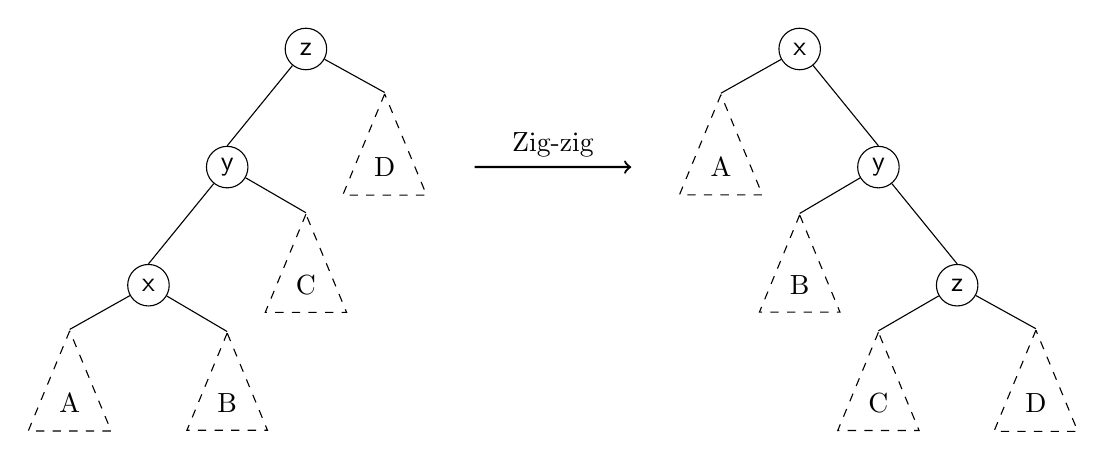
\begin{tikzpicture}[level/.style={sibling distance = 2cm), level distance=1.5cm}]

% Draw the initial tree
\node [tnode] (z) {z}
      [child anchor=north] 
   child{ node [tnode] {y}
      [child anchor=north]
      child{
        node [tnode] {x}
        child { node [subtree] {A} }
        child { node [subtree] {B} }
      }
      child{ node [subtree] {C} }
    }
    child{
       node [subtree] (d) {D} 
    }       
; 

% Draw the result
\node [tnode, right of=z, right=5cm] (xnew) {x}
    [child anchor=north] 
    child{
       node [subtree] (anew) {A} 
    } 
    child {
      node [tnode] {y}
      child { node [subtree] {B} }
      child { node [tnode] (znew) {z}
        [child anchor=north]
        child{ node [subtree] {C} }
        child{ node [subtree] {D} }
      }
    }
; 

\draw[->, shorten <=.75cm, shorten >=.75cm][thick] (d) to[out=0,in=180] node [auto]{Zig-zig} (anew);

\end{tikzpicture}

\begin{tikzpicture}[level/.style={sibling distance = 2cm), level distance=1.5cm}]

% Draw the initial tree
\node [tnode] (z) {z}
      [child anchor=north] 
   child{ node [tnode] {y}
      [child anchor=north]
      child{ node [subtree] {A} }
      child{
        node [tnode] {x}
        child { node [subtree] {B} }
        child { node [subtree] {C} }
      }
    }
    child{
       node [subtree] (d) {D} 
    }       
; 

% Draw the result
\node [tnode, right of=z, right=6cm] (xnew) {x}
    [child anchor=north, level/.style={sibling distance=6cm/2^#1}] 
    child{
      node [tnode] (ynew) {y} 
      child { node [subtree] {A} }
      child { node [subtree] {B} }
    } 
    child {
      node [tnode] {z}
      child { node [subtree] {C} }
      child { node [subtree] {D} }
    }
; 

\draw[->, shorten <=.75cm, shorten >=.75cm][thick] (d) to[out=0,in=180] node [auto]{Zig-zag} (anew);

\end{tikzpicture}

\subsection{Concept}
When we search for $x$, we move it up to the root using the above primitives (any maybe a single rotation).
We will show that the amortized access time is $O(\log n)$.

\subsection{Potential Function}
Let $S(x)=$ size of the subtree rooted at x. Let $r(x)=\log(S(x))$.

\[\Phi(T)=\sum_{x\in T} r(x)\]

\paragraph{Potential of a full binary tree}
$r(x_i)=\frac{n}{2^i}\cdot\log (2^{i-1})$ for each node $x_i$ at depth $i$ where $i$ is 0 at the root.
\[\Phi(T)=\sum_{i=1}^{\log n} \frac{n}{2^i}\cdot\log (2^{i-1}) = n \sum \frac{i-1}{2^i} = \Theta(n) \]

\paragraph{Potential of a string}
\[\Phi(T)=\sum_{i=1}^{n}\log(i)=\Theta(n\log n)\]

\subsection{Amortized Access}

\paragraph{Actual Cost}
We pay the depth to find an element, and half the depth for zigzig and zigzag splaying.

\[cost(\text{zig-zig}) = 2 + \Delta \Phi\]

$r$ changes for $x$, $y$, and $z$. $r'(x) = r(z)$, $r(y)\ge r(x)$, and $r'(x)\ge r'(y)$. Also, $S(x)+S'(z)<S'(x)$.

\[cost(\text{zig-zig}) = 2+r'(x)+r'(y)+r'(z)-r(x)-r(y)-r(z)\]
\[\le r'(x)+r'(z)-2r(x)=(*)\]

Note that the $\log$ function is convex, such that $\frac{\log a + \log b}{2} < \log(\frac{a+b}{2})$ for any $a$, $b$.

\[\frac{r(x)+r'(z)}{2}=\frac{\log S(x) + \log S'(z)}{2} \le \log\left( \frac{S(x)+S'(z)}{2} \right)\]
\[\le \log \frac{S'(x)}{2} = r'(x)-1\]

\[r'(z) \le 2r'(x)-2-r(x)\]
\[(*)\le 3r'(x)-3r(x)\]

\[
cost(\text{zig-zag})\footnote{Not proven in class, and not a particularly interesting proof either...}
\le 2(r'(x)-r(x))\le 3r'(x)-3r(x)
\]

\subparagraph{Cost of splay}
\[
\sum_{
  \begin{matrix}
    \text{zig-zig}\\
    \text{zig-zag}
  \end{matrix}
} cost(op)
\le \underbrace{\sum 3(r'(x)-r(x))}_{\text{series cancels out}}
= 3(r(root)-r(x))
\le 3 \log n
\]

\subsection{Insertion}
Insert $x$ in its correct place, and then splay $x$.

\paragraph{Example: Inserting 13}\ \\
% TODO: figure out how to make the line from 12 to 13 dashed
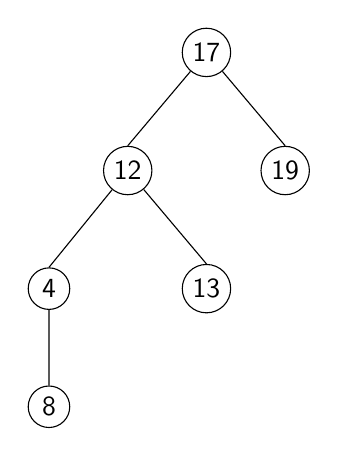
\begin{tikzpicture}[level/.style={sibling distance = 2cm), level distance=1.5cm}]
\node [tnode] (z) {17}
      [child anchor=north] 
    child{
      node [tnode] {12}
      [child anchor=north]
      child{
        node [tnode] {4}
        child { node [tnode] {8} }
      }
      child{
        node [tnode] {13}
      }
    }
    child{
       node [tnode] {19} 
    }       
; 
\end{tikzpicture}

\subsection{Search}
Look for $x$ and splay the last element found while looking.

\subsection{Join}
Combine $T_1$ and $T_2$ where all the elements in $T_1$ are smaller than $T_2$.
Find the largest element $x$ in $T_1$ and splay it. Then connect $T_2$ as the right child of $x$

\subsection{Split}
Given an element $x$, find it in the tree, and splay it. Then return the children.

\subsection{Delete}
Search for $x$, splay it, and then return the join of the children.

\subsection{Weighted analysis}
Let $w(x)$ be some weight function for each node $x$ in the tree.
Instead of using $S(x)$ as the size of the subtree rooted at $x$, let $S(x)=\sum_{y\in T_x} w(y)$.
Note that we've already shown the case where $w(x)=1$ for every $x$, in which case the amortized cost is $O(\log n)$.

\paragraph{staticOPT}
Recall that for a sequence of operations $\sigma$ where $x$ appears $f_x$ times:
\[staticOPT=\Theta\left( \sum \frac{f_i}{m} \log\left(\frac{m}{f_i}\right)\right)\]
\[\text{entropy}=\sum p_i \log \frac{1}{p_i}\]

Let $w(x)=f_x$.
\[amort(splay(x))\le 3(\underbrace{\log(m)}_{\sum f_y=m} - \log(S(x))) \le 3(\log m - \log f_x)\]
\[=O\left(\log \frac{m}{f_x}\right)\]

\[amort(\sigma)=\frac{1}{m}\sum f_x \log \frac{m}{f_x}=\sum \frac{f_x}{m} \log\left(\frac{m}{f_x}\right)\]

\paragraph{Static Finger Theorem}
Let $dist(x,y)=$ the number of elements between $x$ and $y$ (inclusive) on a path through the tree.
For any constant element $f$ the amortized operation cost is $\log(dist(x,f))$. In other words, for any element $x$ the amortized cost is 

\subparagraph{Proof}
Let $w(x)=\frac{1}{dist(x,f)^2}$\footnote{Even Shay admitted he has no idea where in the hell this came from, and that the potential function can become negative, but that it is bound, so it's not that bad}.

\[S(root) \le 2 \sum_{i=0}^{\infty} \frac{1}{i^2}=O(1)\]
\[S(x) \ge w(x) \ge \frac{1}{dist(f,x)^2}\]
\[r(x) \ge -2 \log n\]

Which gives us that the amortized cost is $O(\log dist(x,f))$

\paragraph{Working Set Theorem}
The amortized access time to an element $x$ is $O(\log D)$ where $D$ is the number of distinct elements that have been accessed since the last access of $x$.\footnote{Unproven in the lecture because the weight function is dynamic}

\paragraph{Sequential Access Theorem}
The amortized cost to access each element in order is $O(n)$ without regard to the initial state of the tree.

\paragraph{Dynamic Finger Theorem}
Immediately following $splay(y)$ the amortized cost of $splay(x)$ is $O(\log dist(y,x))$.

\paragraph{$dynamicOPT$ Conjecture}
Splay trees are $O(1)$-competitive with $dynamicOPT$.

\section{Next Week}
So far, we've been looking for setting lower bounds on various static/dynamic optimums in order to prove competition. We will show a lower bound on all binary trees for some sequence of operations, and then show a tree that is $O(\log\log n)$-competitive.

\end{document}
